\subsubsection{reachInner} \label{sec:reachInner}

The operation \operator{reach}, which was introduced in \cref{sec:reach}, computes a tight outer-approximation $\mathcal{R}(t) \supseteq \mathcal{R}^e(t)$ of the exact reachable set $\mathcal{R}^e(t)$ as defined in \eqref{eq:reachSet}. For most cases computing an outer-approximation of the reachable set is sufficient. However, sometimes it also required to compute an inner-approximation $\mathcal{R}^i(t) \subseteq \mathcal{R}^e(t)$ of the exact reachable set: Inner-approximations can be used to prove that a system provably violates a given specification, they are required for conformance testing using \textit{reachset conformance} \cite{Roehm2016}, and they are very useful for controller synthesis where one often has to prove that the controlled system is guaranteed to reach a certain goal set.

The operation \operator{reachInner} computes a tight inner-approximation $\mathcal{R}^i(t) \subseteq \mathcal{R}^e(t)$ of the exact reachable set $\mathcal{R}^e(t)$ as defined in \eqref{eq:reachSet}. Currently, CORA only supports the computation of inner-approximations for the reachable set at certain time-points $t_i$, but not for time intervals $\tau_i = [t_i,t_{i+1}]$. Since some approaches compute an inner-approximation based on the outer-approximation of the reachable set, the operation \texttt{reachInner} returns in some cases both an inner-approximation as well as an outer-approximation of the reachable set.

The syntax for the operation \texttt{reachInner} is:
\begin{equation*}
	\begin{split}
		[\texttt{Rin},\texttt{Rout}] &= \texttt{reachInner}(\texttt{sys},\texttt{params},\texttt{options}), \\
		\texttt{Rin} &= \texttt{reachInner}(\texttt{sys},\texttt{params},\texttt{options}),
	\end{split}
\end{equation*}
with input arguments

\begin{center}
\renewcommand{\arraystretch}{1.3}
\begin{tabular}[t]{l p{13cm} }
	$\bullet$~\texttt{sys} & dynamic system defined by any of the classes in \cref{sec:continuousDynamics}, e.g., \texttt{linearSys}, \texttt{nonlinearSys}, etc. \\
	$\bullet$~\texttt{params} & struct containing the parameter that define the reachability problem. The parameters are identical to those for the operation \texttt{reach} (see \cref{sec:reach}). \\
	$\bullet$~\texttt{options} & struct containing algorithm settings for reachability analysis. Since the settings are different for each type of dynamic system, they are documented in \cref{sec:continuousDynamics}.
\end{tabular}
\end{center}

and output arguments

\begin{center}
\renewcommand{\arraystretch}{1.3}
\begin{tabular}[t]{l p{13cm} }
	$\bullet$~\texttt{Rin} & object of class \texttt{reachSet} (see \cref{sec:reachSet}) that stores the inner-approximations $\mathcal{R}^i(t_i)$ of the reachable set at time points $t_i$. \\
	$\bullet$~\texttt{Rout} & object of class \texttt{reachSet} (see \cref{sec:reachSet}) that stores the outer-approximations $\mathcal{R}(t_i)$ of the reachable set at time points $t_i$ (class \texttt{nonlinearSys} only).
\end{tabular}
\end{center}


Let us demonstrate the operation \texttt{reachInner} by an example:

\begin{center}
\begin{minipage}[t]{0.58\textwidth}
	\footnotesize
	% This file was created by matlab2tikz.
%
\definecolor{mycolor1}{rgb}{0.00000,0.44700,0.74100}%
\definecolor{mycolor2}{rgb}{0.85000,0.32500,0.09800}%
%
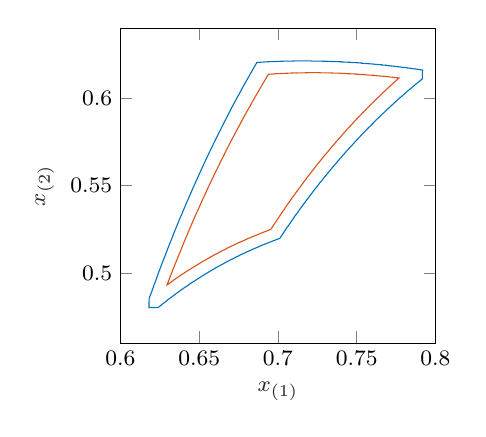
\begin{tikzpicture}
\footnotesize

\begin{axis}[%
width=4cm,
height=4cm,
at={(0in,0in)},
scale only axis,
xmin=0.6,
xmax=0.8,
xlabel style={font=\color{white!15!black}},
xlabel={$x_{(1)}$},
ymin=0.46,
ymax=0.64,
ylabel style={font=\color{white!15!black}},
ylabel={$x_{(2)}$},
axis background/.style={fill=white}
]
\addplot [color=mycolor1, forget plot]
  table[row sep=crcr]{%
0.7884	0.6087\\
0.7853	0.6063\\
0.7822	0.604\\
0.7791	0.6015\\
0.776	0.5991\\
0.77	0.5941\\
0.7699	0.5941\\
0.767	0.5915\\
0.7669	0.5915\\
0.764	0.5889\\
0.7639	0.5889\\
0.761	0.5863\\
0.7581	0.5836\\
0.758	0.5836\\
0.7522	0.5782\\
0.7493	0.5754\\
0.7465	0.5726\\
0.7436	0.5698\\
0.738	0.564\\
0.7353	0.5611\\
0.7352	0.5611\\
0.7298	0.5551\\
0.7297	0.5551\\
0.7271	0.5521\\
0.727	0.5521\\
0.7244	0.549\\
0.7243	0.549\\
0.7191	0.5428\\
0.719	0.5428\\
0.7138	0.5364\\
0.7113	0.5332\\
0.7112	0.5332\\
0.7062	0.5266\\
0.7061	0.5266\\
0.7036	0.5232\\
0.7012	0.5199\\
0.6985	0.519\\
0.6933	0.5172\\
0.6908	0.5163\\
0.6907	0.5163\\
0.6882	0.5153\\
0.6856	0.5143\\
0.6806	0.5123\\
0.6805	0.5123\\
0.678	0.5112\\
0.6755	0.5102\\
0.6755	0.5101\\
0.6731	0.5091\\
0.673	0.509\\
0.6706	0.5079\\
0.6681	0.5068\\
0.6657	0.5056\\
0.6632	0.5044\\
0.6608	0.5032\\
0.6584	0.5019\\
0.656	0.5007\\
0.656	0.5006\\
0.6536	0.4994\\
0.6536	0.4993\\
0.6513	0.4981\\
0.6512	0.498\\
0.6489	0.4967\\
0.6466	0.4953\\
0.6465	0.4953\\
0.6442	0.494\\
0.6442	0.4939\\
0.6396	0.4911\\
0.635	0.4881\\
0.6328	0.4866\\
0.6305	0.4851\\
0.6283	0.4835\\
0.6261	0.482\\
0.6261	0.4819\\
0.6238	0.4803\\
0.6206	0.4803\\
0.6205	0.4804\\
0.6181	0.4804\\
0.6181	0.4837\\
0.6182	0.4838\\
0.6182	0.4855\\
0.6201	0.4901\\
0.6219	0.4947\\
0.622	0.4948\\
0.6238	0.4993\\
0.6238	0.4994\\
0.6257	0.5039\\
0.6257	0.504\\
0.6276	0.5084\\
0.6277	0.5085\\
0.6315	0.5175\\
0.6316	0.5175\\
0.6335	0.5219\\
0.6335	0.522\\
0.6375	0.5308\\
0.6396	0.5351\\
0.6396	0.5352\\
0.6416	0.5395\\
0.6437	0.5438\\
0.6437	0.5439\\
0.6458	0.5481\\
0.6458	0.5482\\
0.65	0.5566\\
0.6522	0.5608\\
0.6522	0.5609\\
0.6543	0.565\\
0.6565	0.5691\\
0.6565	0.5692\\
0.6587	0.5732\\
0.6587	0.5733\\
0.6609	0.5773\\
0.6609	0.5774\\
0.6632	0.5814\\
0.6654	0.5854\\
0.6654	0.5855\\
0.6677	0.5894\\
0.6677	0.5895\\
0.67	0.5934\\
0.67	0.5935\\
0.6723	0.5973\\
0.6723	0.5974\\
0.6746	0.6013\\
0.6747	0.6013\\
0.677	0.6051\\
0.677	0.6052\\
0.6794	0.609\\
0.6794	0.6091\\
0.6818	0.6128\\
0.6818	0.6129\\
0.6842	0.6166\\
0.6842	0.6167\\
0.6866	0.6204\\
0.6896	0.6206\\
0.69	0.6206\\
0.6925	0.6208\\
0.693	0.6208\\
0.6955	0.6209\\
0.696	0.6209\\
0.6984	0.621\\
0.699	0.621\\
0.7014	0.6211\\
0.7021	0.6211\\
0.7044	0.6212\\
0.7086	0.6212\\
0.7104	0.6213\\
0.7212	0.6213\\
0.7214	0.6212\\
0.7281	0.6212\\
0.7282	0.6211\\
0.7314	0.6211\\
0.7333	0.621\\
0.7345	0.621\\
0.7407	0.6208\\
0.7407	0.6207\\
0.7469	0.6205\\
0.7469	0.6204\\
0.75	0.6203\\
0.7532	0.6201\\
0.7532	0.62\\
0.7563	0.6198\\
0.7595	0.6196\\
0.7627	0.6193\\
0.7659	0.6191\\
0.7659	0.619\\
0.7691	0.6188\\
0.7691	0.6187\\
0.7755	0.6181\\
0.7787	0.6177\\
0.7819	0.6174\\
0.782	0.6173\\
0.7852	0.617\\
0.7852	0.6169\\
0.7885	0.6166\\
0.7885	0.6165\\
0.7917	0.6161\\
0.7918	0.6161\\
0.7918	0.6153\\
0.7917	0.6152\\
0.7917	0.6114\\
0.7916	0.6113\\
0.7916	0.611\\
0.7885	0.6087\\
0.7884	0.6087\\
};
\addplot [color=mycolor2, forget plot]
  table[row sep=crcr]{%
0.7741	0.6093\\
0.7685	0.6047\\
0.7657	0.6023\\
0.763	0.5999\\
0.7602	0.5975\\
0.7575	0.5951\\
0.7548	0.5926\\
0.7522	0.5901\\
0.7521	0.5901\\
0.7495	0.5876\\
0.7468	0.585\\
0.7442	0.5825\\
0.7416	0.5798\\
0.739	0.5772\\
0.7364	0.5745\\
0.7339	0.5719\\
0.7314	0.5691\\
0.7313	0.5691\\
0.7288	0.5664\\
0.7238	0.5608\\
0.7214	0.558\\
0.7189	0.5551\\
0.7117	0.5464\\
0.7093	0.5434\\
0.707	0.5404\\
0.7069	0.5404\\
0.7046	0.5374\\
0.7046	0.5373\\
0.7023	0.5343\\
0.6954	0.525\\
0.6932	0.5242\\
0.6911	0.5235\\
0.691	0.5235\\
0.6889	0.5227\\
0.6845	0.5211\\
0.6824	0.5203\\
0.6802	0.5195\\
0.6781	0.5186\\
0.676	0.5178\\
0.6759	0.5178\\
0.6675	0.5142\\
0.6675	0.5141\\
0.6655	0.5132\\
0.6654	0.5132\\
0.6634	0.5123\\
0.6634	0.5122\\
0.6613	0.5113\\
0.6613	0.5112\\
0.6593	0.5103\\
0.6572	0.5093\\
0.6572	0.5092\\
0.6532	0.5072\\
0.6531	0.5072\\
0.6471	0.5039\\
0.6452	0.5028\\
0.6451	0.5028\\
0.6432	0.5017\\
0.6412	0.5006\\
0.6412	0.5005\\
0.6392	0.4994\\
0.6354	0.497\\
0.6353	0.497\\
0.6334	0.4958\\
0.6315	0.4945\\
0.6296	0.4933\\
0.6313	0.4974\\
0.6331	0.5015\\
0.6331	0.5016\\
0.6349	0.5056\\
0.6367	0.5097\\
0.6386	0.5137\\
0.6386	0.5138\\
0.6404	0.5178\\
0.6423	0.5218\\
0.6441	0.5257\\
0.646	0.5297\\
0.6479	0.5336\\
0.6499	0.5375\\
0.6518	0.5414\\
0.6538	0.5452\\
0.6557	0.549\\
0.6597	0.5566\\
0.6618	0.5603\\
0.6618	0.5604\\
0.6638	0.5641\\
0.6659	0.5678\\
0.6658	0.5678\\
0.6679	0.5715\\
0.6742	0.5823\\
0.6742	0.5824\\
0.6764	0.5859\\
0.6763	0.5859\\
0.6785	0.5895\\
0.6829	0.5965\\
0.6828	0.5965\\
0.6851	0.6\\
0.685	0.6\\
0.6873	0.6034\\
0.6873	0.6035\\
0.6917	0.6103\\
0.694	0.6137\\
0.6965	0.6138\\
0.6989	0.614\\
0.7114	0.6145\\
0.7115	0.6144\\
0.714	0.6145\\
0.7165	0.6145\\
0.719	0.6146\\
0.7267	0.6146\\
0.7267	0.6145\\
0.7319	0.6145\\
0.7371	0.6143\\
0.7397	0.6143\\
0.7397	0.6142\\
0.7423	0.6142\\
0.7423	0.6141\\
0.7475	0.6139\\
0.7502	0.6138\\
0.7502	0.6137\\
0.7528	0.6136\\
0.7554	0.6134\\
0.7581	0.6132\\
0.7608	0.6131\\
0.7608	0.613\\
0.7634	0.6128\\
0.7688	0.6124\\
0.7715	0.6121\\
0.7742	0.6119\\
0.7742	0.6118\\
0.7769	0.6116\\
0.7741	0.6093\\
};
\end{axis}
\end{tikzpicture}%
\end{minipage}
\begin{minipage}[t]{0.4\textwidth}
	\vspace{0pt}
	\centering
	\includetikz{./figures/tikz/contDynamics/example_reachInner}
\end{minipage}
\end{center}